\graphicspath{{/Users/brunomedina/Dropbox/Tesis-Egobets/egobets-notas/resources/marco/}}
\chapter{Marco teórico}
\section{La Industria de las Apuestas}
\subsection{La fascinación por los juegos de azar}

Nadie conoce el origen de las apuestas, algunos dicen que todo comenzó con un anónimo paleolítico que rodó unos cuantos huesos para decidir hacia que dirección ir a cazar. Más adelante, los antiguos griegos y etruscos examinarían la forma y  las características del higado de una oveja para tomar las mejores decisiones para su futuro\footnote{Los adivinos llamados ``Arúspices'' eran los encargados de llevar la tarea de precedir el futuro en función de la examinación de las entrañas de varias bestias.}. Siglos después, los romanos usarían los huesos astrágalos de animales como precursores a los dados. \cite{schwartz2013roll}

\begin{figure}[!htb]\centering
   \begin {minipage}{0.85\textwidth}
     \frame{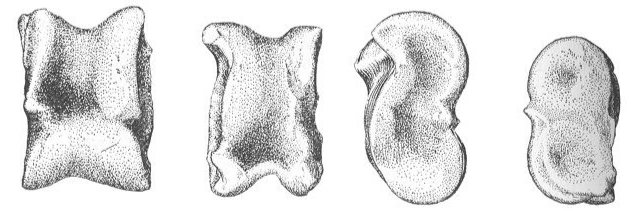
\includegraphics[width=\linewidth]{huesos}}
     \caption{Astrágalos, los predecesores de los dados}\label{Fig:huesos}
   \end{minipage}
\end{figure}

Hoy en día, las apuestas representan uno de los negocios más redituables del mundo. En 2013 se estima que las ganancias brutas de la industria sumaron cuatroscientos cuarenta mil millones de dólares\footnote{Acorde a la empresa de Inteligencia de Mercado ``H2 Gambling Capital'' \cite{economistHouseWins}} (Ver figura~\ref{Fig:gasto-apuestas}) Estados Unidos encabeza la lista como el país que más gasta en apuestas, seguido por China. En la gráfica también se puede observar que los residentes de Australia y Singapur apuestan mucho más agresivamente que cualquier otro. Finalmente, la predicción de que ofrece la firma, propone un gran crecimiento en los casinos y un estimado de más de quinientos mil millones de dólares gastados en apuestas para el 2018.


\begin{figure}[!htb]\centering
   \begin {minipage}{0.85\textwidth}
     \frame{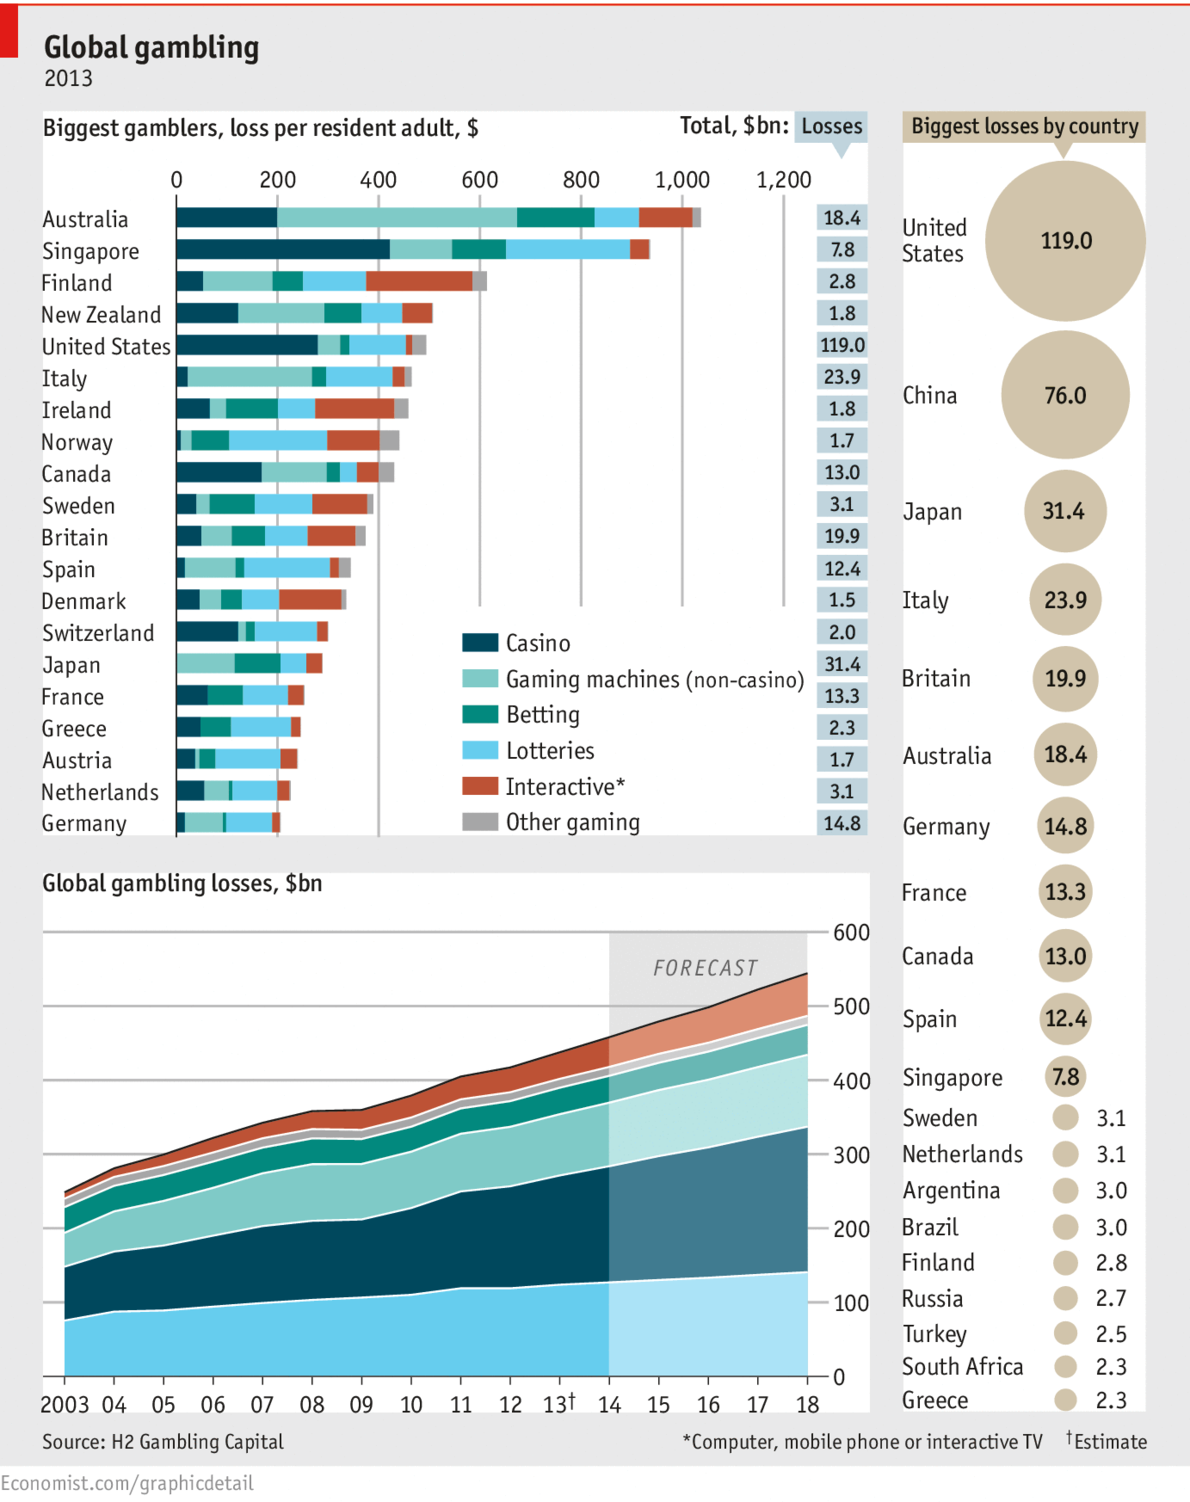
\includegraphics[width=\linewidth]{apuestas}}
     \caption{Miles de millones de dólares en apuestas}\label{Fig:gasto-apuestas}
   \end{minipage}
\end{figure}

Con estos datos, la importancia de la industria de las apuestas en el mundo se vuelve evidente. De la misma forma, en el ámbito de apuestas en línea, la firma KPMG \cite{kpmgOnlineGaming} presenta datos más focalizados; a pesar de la falta de regulación y las leyes en contra de los casinos en línea, el mercado global de apuestas en línea creció un cuarenta y dos por ciento de 2008 (Veintún mil doscientos millones de dólares) a 2012 (Treinta mil millones de dólares), este crecimiento es notablemente superior al quince por ciento que se propuso para el crecimiento del total de la industria de apuestas para el mismo periodo.

Específicamente en Estados Unidos, Goldman Sachs valoró en 2009 que el mercado de apuestas en línea en caso de ser legalizado\footnote{Actualmente se les prohíbe procesar cargos relacionados a casinos en línea a los bancos y a las compañías de tarjetas de credito. Gracias al``Unlawful Internet Gambling Enforcement Act of 2006'' (UIGEA)} podría valer hasta doce mil millones de dólares \cite{goldmanParty}.En este mismo documento de KPMG \cite{kpmgOnlineGaming}, México se propone como un mercado potencialmente lucrativo. Una de las principales razones es la legislación que permite el juego en línea\footnote{En 2004, la Ley Federal de Juegos con Apuestas y Sorteos permitió y reguló los Juegos en Línea}. La otra razón, el valor del mercado mexicano del juego en línea se estima en cuatro mil seiscientos millones de dólares \cite{yogonet}.

\subsection{La casa siempre gana}

\begin{chapquote}{Adam Smith, \textit{Filósofo}}
	``No hay proposición más cierta en matemáticas que la siguiente: Entre más boletos [de lotería] compre, más probabilidades tiene de ser un perdedor. Compre todos los boletos de la lotería y pierda con certeza; cuanto más boletos compre, más cerca estará de esta certeza''
\end{chapquote}

El principio básico detrás de un casino es muy sencillo: \emph{la ventaja de la casa}. Cada uno de los juegos que ofrece el casino tiene detrás un robusto sustento matemático que, a pesar de hacerlos aparentar como juegos justos, le confiere a la casa una ventaja porcentual sobre el conjunto de jugadores. Al final del día, esta ventaja y la ley de los grandes números, le garantizan a los casinos que a largo plazo tendrán suficientes ganancias para subsistir, mantener su operación y gozar de utilidades sorprendentes. Sin embargo, no hay que olvidar que los fenomenos estudiados siguen siendo producto del azar, por lo que una buena racha de algunos ``Grandes Apostadores'' podría llegar a asustar aun a los dueños  más racionales de casinos \cite{hannum2005practical}.



Según Hannum \cite{hannum2005practical} hay dos grandes razones por las que la gente apuesta:

\begin{enumerate}
	\item \textbf{Entretenimiento.} Un individuo podría utilizar mil pesos para ir a un casino o a un concierto. Si la ventaja de la casa es muy grande y la persona pierde su dinero rápidamente, entonces la experiencia del entreteniminto del casino no sería apreciada por el jugador. Por el otro lado, si el casino logra entretener a la persona por una tarde mientras le regala bebidas y comida, entonces puede que este individuo repita la experiencia y nunca más asista a un concierto.
	\item \textbf{Cambio de Vida.} Si una persona ahorrara cien pesos semanalmente, al final del un año tendría cinco mil doscientos pesos. Pero si ese dinero lo gastara para comprar boletos de lotería, tendría la posibilidad de ganarse cuarenta millones de pesos. Claramente la probabilidad es muy cercana a cero; sin embargo, este gasto podría ser visto por esta persona como una única oportunidad para cambiar su vida.

\end{enumerate}

\emph{La ventaja de la casa}, se puede entender mejor analizando cada uno de los juegos que ofrece el casino y las probabilidades de ganar que tienen los jugadores. Tómese el juego de la ruleta americana:\footnote{El juego de la ruleta americana consiste en 18 casillas rojas, 18 casillas negras y 2 casillas sin color sobre las cuales, al girar de manera aleatoria, cae una pelotita. Los jugadores apuestan sobre la posición final de la pelotita.}
Al tener $38$ casillas, si un jugador apuesta sobre el color negro (i.e. que la pelotita caiga sobre alguna de las casillas negras) entonces tenemos que la probabilidad de que el jugador gane la apuesta es de:\\
\[p\{\text{La pelotita caiga en casilla negra}\} = \frac{\text{\# casillas negras}}{ \text{\# casillas totales}}  = \frac{18}{38}\]\\

Afortunadamente para la casa, hay $2$ casillas que no son color negro ni rojo, por lo que de las $38$ sólo $36$ casillas tienen estos colores. Entonces, la probabilidaad de que la pelotita evite estos colores es la siguiente:

\[p\{\text{La pelotita no caiga ni en casillas rojas ni en negra}\} =\] 
\[\frac{\text{\# casillas totales - (\# casillas rojas + \# casillas negras)}}{ \text{\# casillas totales}}  =\]
\[\frac{38-18-18}{38} = \frac{2}{38}  \]

Estos $\frac{2}{38}$ son la ventaja de la casa, ya que cuando un jugador apuesta al color negro en la ruleta y acierta, recibe la misma cantidad de dinero que podría perder. Sin embargo, apostó a ganar con una probabilidad de $\frac{18}{38}$, pero la probabilidad de perder la apuesta es igual a $1 - \frac{18}{38} = \frac{20}{38}$. Este detalle hace importante ver el valor esperado que tiene esta apuesta para el jugador:
\[E[\text{Apostar }k\text{ pesos al color negro}] = k  \cdot   p\{\text{La pelotita caiga en casilla negras}\} \]
\[- k  \cdot   p\{\text{La pelotita no caiga en casilla negra}\} = k \cdot \frac{18-20}{38}= - k \cdot \frac{2}{38}\]

Dado que siempre que se apuesta $k>0$, esto implica que:
\[E[\text{Apostar }k\text{ pesos al color negro}] = - k \cdot \frac{2}{38} < 0; \forall k \in \mathbb{N} \]
Este resultado quiere decir que a la larga el jugador \textbf{siempre} va a terminar perdiendo dinero.
En un principio, $\frac{2}{38}$ de probabilidad pareciera poco, pero al multiplicarlo por la gran cantidad de jugadores y apuestas que se realizan en los casinos el monto final se vuelve exorbitante.

Este sencillo ejercicio ejemplifica como todos los juegos que se tienen en los casinos ofrecen una ventaja para la casa. Es interesante mencionar, que aparte de los juegos de azar como la ruleta, hay juegos que obligan al jugador a tener cierta habilidad para no perder su dinero tan rápidamente, este es el caso de juegos como el Blackjack que le dan a la casa ventajas más pequeñas al enfrentarse a jugadores expertos. La ventaja de la casa sustenta las ganancias del casino, sin embargo calcular esta ventaja puede llegar a ser  complicado y requerir un análisis matemático mucho más sofisticado e incluso se puede llegar a necesitar programar el juego para correr simulaciones y estimar estas probabilidades.

\begin{table}[ht]
\centering
\resizebox{\textwidth}{!}{%
\begin{tabular}{|l|c|}
\hline
\textbf{Juego}                            & \textbf{Ventaja de la Casa} \\ \hline
Ruleta (con doble cero)                   & 5.3\%                       \\ \hline
Dados (pass/come)                         & 1.4\%                       \\ \hline
Dados (pass/come con momios dobles)       & 0.6\%                       \\ \hline
Blackjack - jugador promedio              & 2.0\%                       \\ \hline
Blackjack - 6 barajas, estrategia básica  & 0.5\%                       \\ \hline
Blackjack - una baraja, estrategia básica & 0.0\%                       \\ \hline
Baccarat (sin apuestas de empate)         & 1.2\%                       \\ \hline
Caribbean Stud                            & 5.2\%                       \\ \hline
Let It Ride                               & 3.5\%                       \\ \hline
Poker de tres cartas                      & 3.4\%                       \\ \hline
Pai Gow Poker (ante/play)                 & 2.5\%                       \\ \hline
Tragamonedas                              & 5\% - 10\%                  \\ \hline
Video Poker                               & 0.5\% - 3\%                 \\ \hline
Keno (promedio)                           & 27.0\%                      \\ \hline
\end{tabular}
}
\caption{Ventajas de la casa para juegos populares de casino \cite{hannum2005practical}}
\label{ventaja-casa}
\end{table}

Finalmente, aun sin la ventaja de la casa se deber recordar que existe un famoso problema y su corolario que garantizan que la casa siempre gane: \emph{La ruina del Jugador} \cite[p.~95-99]{ross2006first}. Este problema enfrentado por varios famosos matemáticos\footnote{Se dice que Blaise Pascal se lo planteó a Pierre Fermat en 1656. Después fue replanteado a Christian Huygens y finalmente James Bernoulli resolvió en su forma general como el problema de la ``Duración de Juego''} deja la siguiente lección: La probabilidad de un jugador perder todo su dinero es igual al cociente entre la cantidad de dinero de su oponente sobre la suma de la cantidad de dinero de ambos: $p_1 = \frac{n_2}{n_1 + n_2}$ donde $p_1$ es la probabildad de ganar del jugador $1$ y $n_i$ es la cantidad de dinero que va a apostar el jugador $i$. Desafortunadamente, usualmente  la casa tendrá más dinero para apostar que el jugador.


\subsection{Apuestas deportivas}

\subsection{La gran ventaja}

A diferencia de las máquinas tragamonedas y los juegos de mesa de los casinos, las apuestas deportivas tienen una gran ventaja: \textbf{los resultados no son completamente aleatorios}. Hannum menciona en su libro: \emph{``La ventaja de la casa existe para casi todas las apuestas en un casino (ignorando las salas de Poker y las apuestas deportivas donde algunos pocos profesionales pueden vivir de de las apuestas)''} \cite{hannum2005practical} 

Existen dos grandes mercados en esta rama de las apuestas \cite{chung2010empirical}:
\begin{itemize} 
	\item \emph{Bookies.} El corredor publica los momios de cada apuesta y cobra una comisión por cada una que recibe. A los jugadores se les promete un pago fijo que va en función de los momios publicados al momentos de hacer sus apuestas.
	\item \emph{Sistema parimutual.} En este mercado no existen los corredores, ni los momios. El pago que reciben los jugadores depende de la cantidad de dinero recopilada por todas las apuestas recibidas. Por lo tanto, las ganancias de los jugadores no están determinadas hasta que todas las apuestas se reciben.
	\end{itemize}

El mercado de estudio de este trabajo es el de los ``bookies'' o corredores de apuestas. Sin embargo, bajo las condiciones adecuadas la asesoría de apuestas podría facilmente ser aplicada al mercado parimutual\footnote{Por ejemplo en una quiniela los otros participantes poseen menos información o son más inexpertos que el jugador usando Egobets}.

Los momios de los bookies han sido cuestionados en eficiencia\footnote{La eficiencia de mercado no es un tema que se profundize en este documento sin embargo se pueden revisar a Sauer \cite{sauer1998economics} y Williams \cite{williams1999information} donde se explica más de anomalías como el ``sesgo favorite-longshot'' que implica que las apuestas a los favoritos generan un mayor retorno que las ``apuestas a longshots'' (apuestas arriesgadas).  } e incluso se han realizado varios estudios proponiendo un nuevo mercado de tipo ``doble subasta''\footnote{Consiste en tener compradores y vendedores fijando los precios, cuando dos de ellos coinciden, se lleva acabo la transacción. Referirse a Ozgit\cite{ozgit2005posted} }

Sin importar el mercado, es importante que se recuerde el hecho de que nadie conoce las probabilidades reales que tienen los distintos resultados de los partidos. Este hecho hace que los ``bookies'' tengan que confiar en sus propios libros e investigaciones para estimar las probabilidades de los partidos. Este punto es básico en la creación de Egobets, ya que el hecho de que las probabilidades sean desconocidas da lugar a que Egobets estime probabilidades mucho más cercanas a las reales, consiguiendo con esto valiosos puntos porcentuales que se podrían traducir en ganacias.


% \subsubsection{Inferencia Estadística}
% \subsubsection{Teoría de la Información}
% \subsubsection{Sistemas de Predicción}



\section{Internet}
\subsection{Contribuyendo con un granito de arena}
La era de la información nos golpeo tan fuerte, que ahora es imposible la vida sin nuestros sistemas de información y nuestros dispositivos de conexión. Gracias a las computadoras y las redes, hemos redefinido nuestra imaginación, hemos creado un espacio que expande nuestra mente y nuestra capacidad, nuestras barreras se han alejado más y ahora nuestra conciencia como especie humana, crece en tasas inimaginables. Los monopolios de la información se han ido disolviendo, permitiendo a la sociedad una mayor participación y voz.

Internet es un organismo vivo y hambriento, con el que convivimos de manera simbiótica y nos une como especie. Es un espacio de comunicación y entendimiento. Nunca pudo haber existido algo más majestuoso y poderoso. La verdadera trascendencia del ser, vendrá con la evolución de la conciencia de la sociedad.

Con esta idea en mente fue diseñado y desarrollado Egobets, un sistema que aporta a la comunidad en internet información últil para la toma de mejores decisiones. Y a su vez, esta información, proviene del procesamiento de varias fuentes de información que otros aportan al internet. El ideal detrás: un conjunto de círculos virtuosos que pongan al alcance de cualquier persona la información más precisa y útil acerca de cualquier tema que se pueda pensar.

\subsection{Computación en la Nube}

El sistema usa la nube para ofrecer sus servicio a los usuarios, se puede decir que el software corre en un esquema tipo ``SaaS''\footnote{Software as a Service. ``Es el más conocido de los niveles de cómputo en la nube. El SaaS es un modelo de distribución de software que proporciona a los clientes el acceso a éste a través de la red (generalmente Internet). De esta forma, ellos no tienen que preocuparse de la configuración, implementación o mantenimiento de las aplicaciones, ya que todas estas labores se vuelven responsabilidad del proveedor. Las aplicaciones distribuidas a través de un modelo de Software como Servicio pueden llegar a cualquier empresa sin importar su tamaño o ubicación geográfica.'' \cite{computoNube}}, esto implica que el usuario simplemente ingresa a su cuenta en un navegador de internet y puede ver las asesorías para sus apuestas.  
Del artículo ``Cómputo en Nube: Ventajas y Desventajas'' de Martínez y Gutiérrez \cite{computoNube}  se retoman las siguentes ventajas de este paradigma:
\begin{itemize}
	\item \textbf{Costos.} Podría ser la ventaja más atractiva que presenta el cómputo en la nube, y si no lo es, al menos es la más evidente de todas las que ofrece esta tecnología. Al dejar la responsabilidad de la implementación de la infraestructura al proveedor, el cliente no tiene que preocuparse por comprar equipos de cómputo, capacitar personal para la configuración y mantenimiento de éstos, y en algunos casos, por el desarrollo del software. Además el usuario de estos servicios únicamente paga por los recursos que utiliza, permitiéndole diseñar un plan de pago normalmente a partir del tiempo en que éste se utiliza (memoria, procesamiento, almacenamiento).
	
	\item \textbf{Competitividad.} Al no tener que adquirir equipos costosos, las pequeñas empresas pueden tener acceso a las más nuevas tecnologías a precios a su alcance pagando únicamente por consumo. De este modo las organizaciones de cualquier tipo podrían competir en igualdad de condiciones en áreas de TI con empresas de cualquier tamaño. La ventaja competitiva no está en aquel que tiene los recursos de cómputo sino en quien los emplea mejor.
	
	\item \textbf{Disponibilidad.} El proveedor está obligado a garantizar que el servicio siempre esté disponible para el cliente. En este sentido, la virtualización juega un papel fundamental, ya que el proveedor puede hacer uso de esta tecnología para diseñar una infraestructura redundante que le permita ofrecer un servicio constante de acuerdo a las especificaciones del cliente.


	\item \textbf{Abstracción de la parte técnica.} Como se mencionó al hablar de costos, el cómputo en la nube permite al cliente la posibilidad de olvidarse de la implementación, configuración y mantenimiento de equipos; transfiriendo esta responsabilidad al proveedor del servicio.

	\item \textbf{Acceso desde cualquier punto geográfico.} El uso de las aplicaciones diseñadas sobre el paradigma del cómputo en la nube puede ser accesible desde cualquier equipo de cómputo en el mundo que esté conectado a Internet. El acceso normalmente se hace desde un navegador web, lo que permite a la aplicación ser utilizada no únicamente desde una computadora de escritorio o una computadora portátil, sino que va más allá, permitiendo al usuario hacer uso de la aplicación incluso desde dispositivos móviles como smartphones.
	
	\item \textbf{Escalabilidad.} El cliente no tiene que preocuparse por actualizar el equipo de cómputo sobre el que se está corriendo la aplicación que utiliza, ni tampoco por la actualización de sistemas operativos o instalación de parches de seguridad, ya que es obligación del proveedor del servicio realizar este tipo de actualizaciones. Además, éstas son transparentes para el cliente, por lo que la aplicación debe de continuar disponible para el usuario en todo momento aún cuando se esté realizando el proceso de actualización del lado del proveedor. Las actualizaciones y nuevas funcionalidades son instaladas prácticamente de manera inmediata.
	
	\item \textbf{Disponibilidad.} El proveedor está obligado a garantizar que el servicio siempre esté disponible para el cliente. En este sentido, la virtualización juega un papel fundamental, ya que el proveedor puede hacer uso de esta tecnología para diseñar una infraestructura redundante que le permita ofrecer un servicio constante de acuerdo a las especificaciones del cliente.
	
\end{itemize}

\subsection{Ingeniería de Software}









\section{Ligas europeas de futbol}
El nivel de juego de los clubes europeos es sorprendente, tanto en la cancha como fuera de ella los Clubes de futbol de las ligas europeas hacen las cosas mejor que ningún otro. Ofrecen partidos de alta calidad, con jugadas complejas y rápidas que proveen de un espectáculo como ningún otro. Además de que la infraestructura, adminsitración y los recursos financieros con los que cuentan son envidiables. Y es por estos motivos que sus niveles de audiencia y la cantidad de sus fanáticos han llegado a niveles impresionantes. Las ligas europeas son en el mundo del futbol: \emph{El modelo a seguir.}


Además de todas las cualidades con las que cuentan estas ligas, se tiene una premisa muy interesante incita el enfoque en ellas: La consistencia que tienen los equipos más populares de cada liga para conseguir victorias sobre los equipos más modestos y su habilidad para siempre permanecer en los mejores lugares de la tabla de posiciones. 

\subsection{Bundesliga (Alemania)}


Fundada el 28 de Julio de 1962 en la convención anual de la \emph{DFL Deutsche Fußball Liga GmbH}, la primer temporada se jugó en 1963. La liga evolucionó en función de la reunificación de Alemania y la integración de la liga del Este \cite{hesse2003tor} Hoy en día la \emph{Bundesliga} es conocida como una de las ligas con mayor afluencia en sus partidos, en la temporada 2011/12 hubo un promedio de 44,293 espectadores por partido. Se vendieron 18.8 millones de entradas en total.

\begin{figure}[!htb]\centering
   \begin {minipage}{0.4\textwidth}
     
\includegraphics[width=\linewidth]{logo-bundesliga}
   \end{minipage}
\end{figure}
\begin{chapquote}{Gary Lineker, \textit{ex-futbolista inglés.}}
	``El fútbol es un deporte que inventaron los ingleses, que lo saben jugar los brasileños y en el que siempre ganan los alemanes.''
\end{chapquote}


La \emph{DFL} se encarga de la operación de las ligas de futbol: \emph{Bundesliga} y \emph{2. Bundesliga}; que son las más importantes de Alemania. Cuenta con treinta y seis clubs de futbol los cuales juegan se dividen en ambas divisiones (Ver~\cref{sec:equipos-ger}) Todos miembros de la Asociación  de la Liga cuentan con una licencia\footnote{Cada temportada todos los clubs deben cumplir los criterios deportivos, legales, administrativos, financieros y de infraestructura del Lizenzierungsordnung (LO) y sus respectivos apéndices} para poder jugar y deben seguir los sistemas de entrenamiento y procedimientos disciplinarios.

Dieciocho equipos juegan en cada división, cada equipo juega una vez de local y otra de visitante contra cada uno de los otros diecisiete equipos de la liga. Esto significa que al ser $n=18$ equipos se tienen $\sum\limits_{i=1}^{n-1} i= \sum\limits_{i=1}^{17} i= 153 $ partidos en una temporada. Al término de estos partidos se calculan los puntos que cada equipo tiene y se hace la tabla de posiciones, los dos peores equipos de la \emph{Bundesliga} son intercambiados con los dos mejores de la \emph{2. Bundesliga}. Mientras que el tercer mejor equipo de la \emph{2. Bundesliga} disputa un partido con el tercer peor equipo de la \emph{Bundesliga} para decidir quien se queda en la primera división. Análogamente, el equipo con más puntos se vuelve el campeón de la liga.

Los puntos de la tabla son dados por las victorias de cada equipo, una victoria suma tres puntos a la tabla; las derrotas o empates no suman nada. Si en la tabla hay equipos con la misma cantidad de puntos, para el desempate se deben consideran criterios como: diferencias de goles, cantidad de goles anotados en la temporada,  diferencia de goles que resulten de los partidos jugados entre ellos y la cantidad de goles como visitantes. Si todos estos criterios no deciden el desempate, se deberá jugar un partido en una cancha neutral para decidir su posición en la tabla.

La regulación de la cantidad de jugadores extranjeros en los equipos sigue la regulación d ela UEFA desde el 21 de Diciembre del 2005. Actualmente hay 977 jugadores con un contrato profesional, 503 en la \emph{Bundesliga} y 474 en la \emph{2. Bundesliga}. El cuarenta y siete por ciento de la primera división son extranjeros (234 jugadores) y el treinta y seis por ciento  en la segunda liga (171 jugadores)

En total, 43 clubs han ganado la Bundesliga desde su fundación. Los tres equipos con más campeonatos son: \emph{FC Bayern Munich} con 23 títulos, \emph{BFC Dynamo Berlin} con 10 y \emph{1. FC Nürnberg} con 9. Los tres máximos goleadores de la liga son: \emph{Ger Müller} (1965-1979) con 365 goles, \emph{Klaus Fischer} (1968-1988) con 268 y \emph{Jupp Heyncke}s con 220. \cite{bundesliga}

\subsection{Liga BBVA (España)}

La Primera División de España comenzó a disputarse en la temporada 1928-29, siendo el FC. Barcelona el primer equipo que se proclamó Campeón. Hasta ese momento, el fútbol español se organizaba en torno al Campeonato de España. Las primeras temporadas se disputaron con los primeros campeones y subcampeones del Campeonato de España. Conocida hoy en día como la \emph{Liga BBVA}\footnote{Nombre proveniente del patrocinio del Banco Bilbao Vizcaya Argentaria. Segunda División ahora se conoce como la \emph{Liga Adelante}. Curiosamente la Segunda División solía tener el nombre de \emph{Liga BBVA} } (por motivos de patrocinio, es considerada hoy en día como la liga de más fuerte del mundo y de mayor importancia. \cite{strongest-league}

\begin{figure}[!htb]\centering
   \begin {minipage}{0.5\textwidth}
     
\includegraphics[width=\linewidth]{logo-bbva}
   \end{minipage}
\end{figure}

La Liga de Fútbol Profesional (LFP) se fundó el 26 de julio de 1984. Es una asociación deportiva integrada por todas las sociedades anónimas deportivas y clubes de fútbol de Primera y Segunda División que participan en competiciones oficiales profesionales de España. La LFP forma parte de la Real Federación Española de Fútbol pero tiene autonomía jurídica en su organización y funcionamiento. 

En la actualidad, la Liga de Fútbol Profesional está formada por un total de 42 equipos: 20 en Primera División y 22 en Segunda División (Ver~\cref{sec:equipos-esp}). Igual que la liga Alemana, cada equipo juega una vez de local y otra de visitante contra cada uno de los otros diecinueve equipos de la liga. Esto significa que al ser $n=19$ equipos se tienen 190 partidos en una temporada. Con estas 38 jornadas los equipos suman puntos en la tabla de posiciones, los primeros 3 entran a la fase de grupos de la \emph{Liga de Campeones de la UEFA}. Los últimos tres equipos en la tabla de posiciones descienden a la \emph{Liga Adelante}, mientras que los mejoes 2 de la Segunda División suben a Primera. El tercer ascenso a Liga BBVA es el ganador de un mini torneo entre el tercer vs quinto y cuarto vs sexto mejor clasificados.

Cada victoria suma tres puntos al Club vencedor, en caso de empate ambos equipos se llevan un punto. Las reglas de desempate son las siguientes: 
\begin{itemize}

	\item El que tenga una mayor diferencia entre goles a favor y en contra según el resultado de los partidos jugados entre ellos.

	\item El que tenga la mayor diferencia de goles a favor teniendo en cuenta todos los obtenidos y recibidos en el transcurso de la competición.

	\item El club que haya marcado más goles.

\end{itemize}

En caso de que haya tres equipos o más empatados se siguen los siguientes criterios para el desmpate:

\begin{itemize}

	\item La mejor puntuación de la que a cada uno corresponda a tenor de los resultados de los partidos jugados entre sí por los clubes implicados.

	\item La mayor diferencia de goles a favor y en contra, considerando únicamente los partidos jugados entre sí por los clubes implicados.

	\item La mayor diferencia de goles a favor y en contra teniendo en cuenta todos los encuentros del campeonato.

	\item El mayor número de goles a favor teniendo en cuenta todos los encuentros del campeonato.

	\item El club mejor clasificado con arreglo a los baremos de fair play.

\end{itemize}

Se inscriben 25 jugadores cada temporada a cada Club, de los que 3 pueden ser ajenos a la Unión Europea. Sin embargo, todos aquellos que se puedan nacionalizar por sus lazos familiares pueden jugar en el equipo sin ocupar una plaza de extracomunitaria.

59 equipos han jugado en esta ligas desde su comienzo. Los únicos 3 que nunca han descendido son: Athletic Club, FC Barcelona y Real Madrid CF. Los campeones máximos son \emph{Real Madrid CF} con 32 títulos, \emph{FC Barcelona} con 22 y \emph{Club Atlético Madrid} con 10. Loa goleadores más prolíficos son: \emph{Telmo Zarra} (1921-2006) con 251 goles, \emph{Lionel Messi} (1987) con 250 y \emph{Hugo Sánchez} (1958) con 234. \cite{primera}

\subsection{Ligue 1 (Francia)}

Fundada el 11 de septiembre de 1932 bajo el nombre de \emph{National} que después cambió a \emph{Division 1}

\begin{figure}[!htb]\centering
   \begin {minipage}{0.5\textwidth}
     
\includegraphics[width=\linewidth]{logo-ligue1}
   \end{minipage}
\end{figure}


\subsection{Premier (Inglaterra)}

La \emph{DFL Deutsche Fußball Liga GmbH} se encarga de la operación de la \emph{Bundesliga} y \emph{2. Bundesliga}, las más importantes ligas de futbol de alemania. Cuenta con treinta y seis clubs 


\subsection{Serie A (Italia)}

La \emph{DFL Deutsche Fußball Liga GmbH} se encarga de la operación de la \emph{Bundesliga} y \emph{2. Bundesliga}, las más importantes ligas de futbol de alemania. Cuenta con treinta y seis clubs 





